\chapter{Project}\label{ch:project}

This chapter is devoted to the description of the general architectures, 
and specific algorithms.


\section{Logical architecture}

The logical architecture is composed by the following component:
\begin{itemize}
    \item \textbf{Web Service} a node of a peer-to-peer layer that 
        provides environment primitives to the car processes (list of adjacent cars) and, 
        at the same time, can send queries to the DB component and exposes an API for the 
        clients.
    \item \textbf{Client} a simple web page used to monitoring the simulation state; 
        uses the web service APIs to render a graphic interface that must 
        be constantly syncronized.
    \item \textbf{Car} a process that is the abstraction/simulation of a real car; 
        \begin{itemize}
            \item it can become a leader in order to schedule the crossing order for the next turn
            \item it must check the health state of the other adjacent cars 
                (calls the tow truck in case of failure)
            \item it can see environment details calling a web service 
            \item it have to syncronize its local timing using Berkeley algorith
        \end{itemize}
    \item \textbf{Distributed DBMS}, an instance of Mnesia DBMS distributed 
        on each container in order increase redundancy and robustness. 
    \item \textbf{Docker Container} wraps one or more car and/or web service instances 
        and is designed to be interconnected with all others containers 
    \end{itemize}


\section{Protocols and algorithms}

We provide a simplified sequence of UML (sequence) diagrams in order to describe the workflow/communication patterns.

\begin{center}
    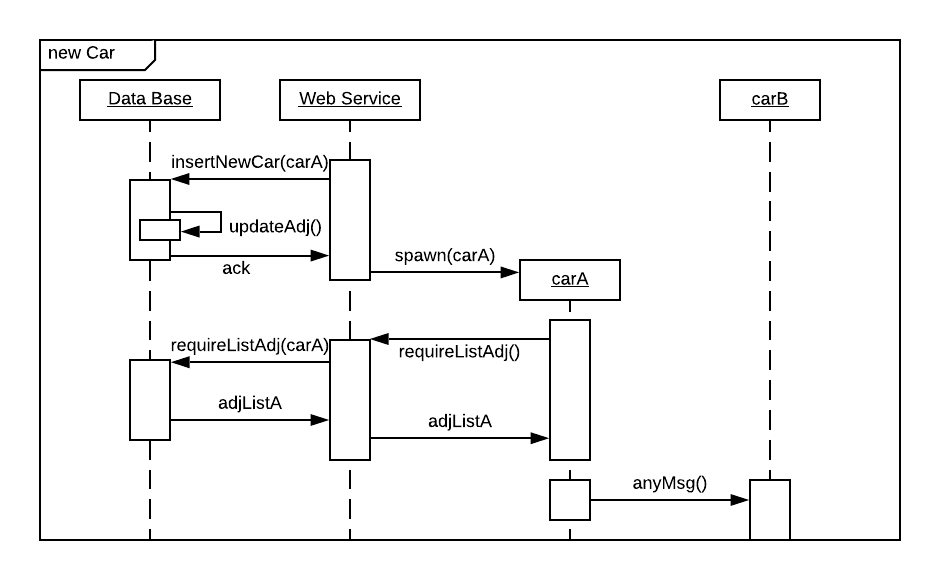
\includegraphics[scale=0.8]{assets/ds2019_1.png}
    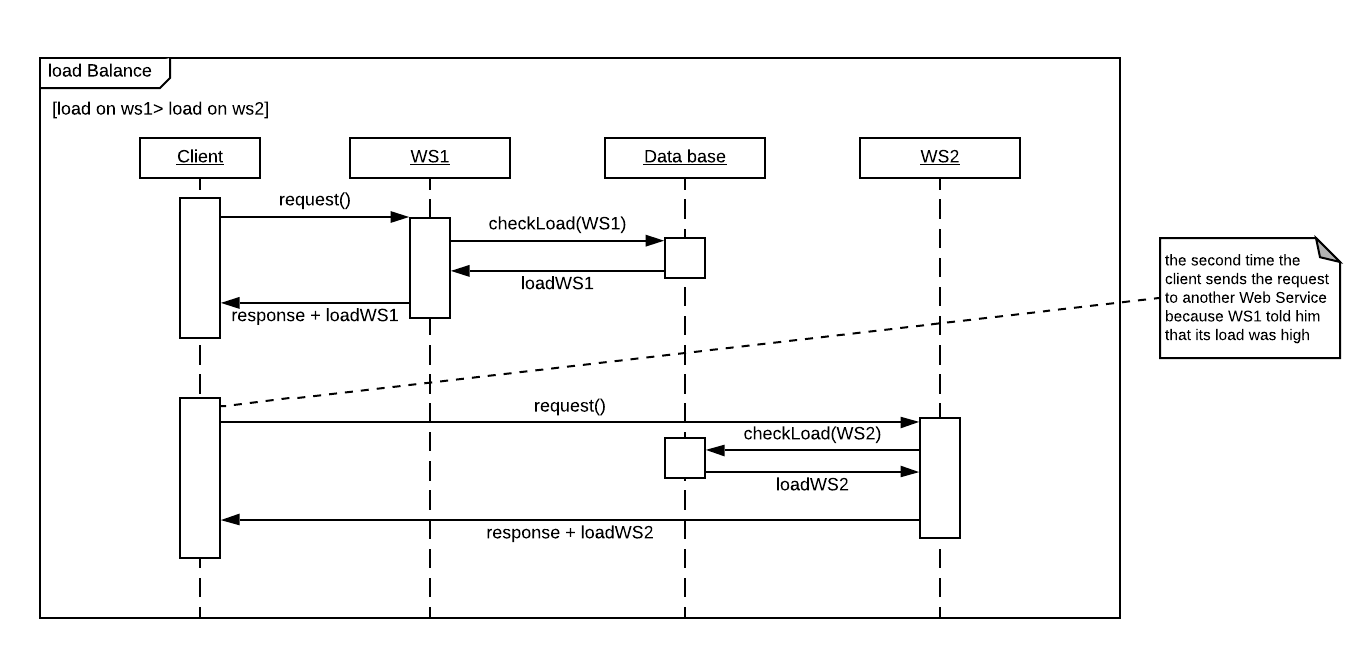
\includegraphics[scale=0.6]{assets/ds2019_2.png}
    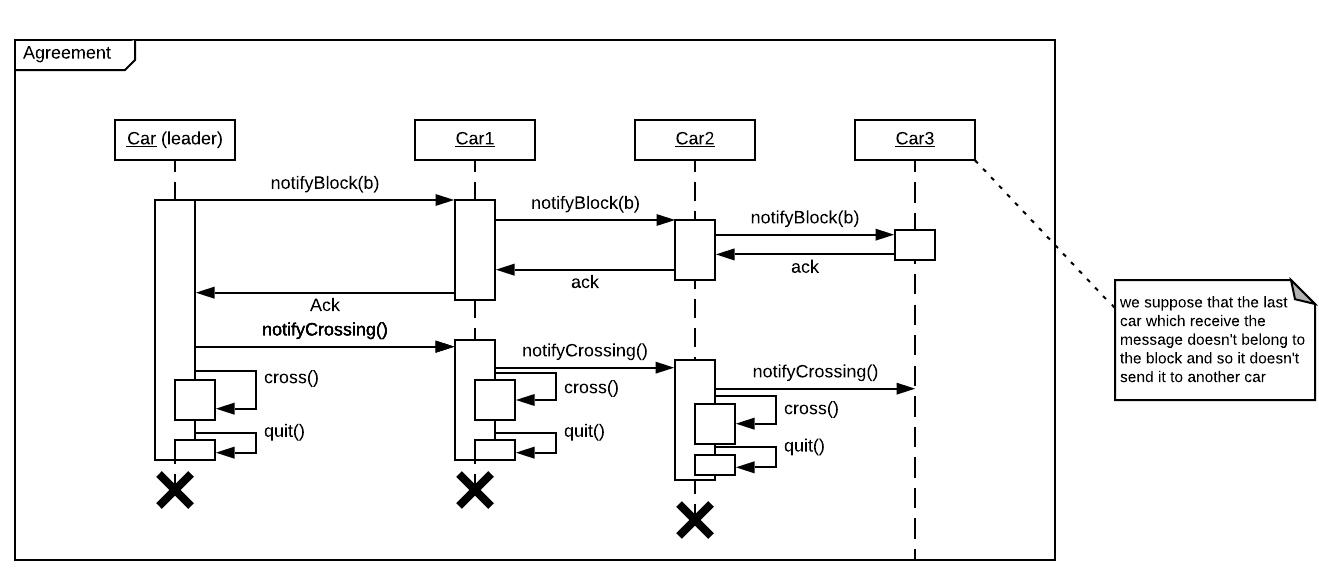
\includegraphics[scale=0.6]{assets/ds2019_3.png}
    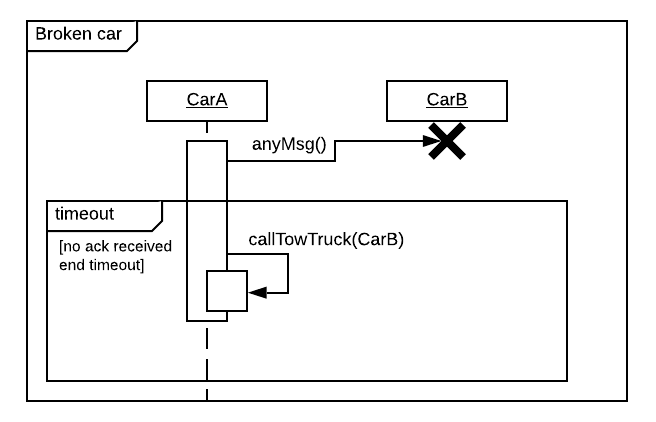
\includegraphics[scale=0.9]{assets/ds2019_4.png}
    %\captionof[figure]{a}
\end{center}

We have used the Berkeley algorithm in order to syncronize new spawned car processes.


\section{Physical architecture and deployment}

The deployment and start up consists in the following steps:
\begin{enumerate}
    \item Get the ssh credentials of each computer involved in the simulation
    \item Execute a launcher bash script that will open an ssh tunnel with each computer and 
        raise the Docker Containers with an arbitrary number of web services 
    \item A random generator or a test procedure inserts into the DB a simulation schedule
        (the web service p2p layer starts automatically the simulation)
    \item With a web browser any client can connect to the web service API and monitoring 
        the simulation state   
\end{enumerate}

The code required for the simulation is taken directly from the project repository hosted on 
GitHub~\cite{2}.


\section{Development plan}

The proposed architecture is a classical \textbf{three-tier architecture} 
(client, web service and DBMS).
